\section*{Step 4}

\begin{custombox}[label={box:Q4}]{Step 4}
	Calculate and analyze the metrics you have listed in ‘1’ above. Analyze them across the datasets and methods. Create appropriate plots and explain the trends, if any, and the outcomes of your analysis. What can you conclude (Please don’t state the obvious !!)
\end{custombox}

\subsection*{Dataset 1}

\begin{figure}[H]
	\centering
	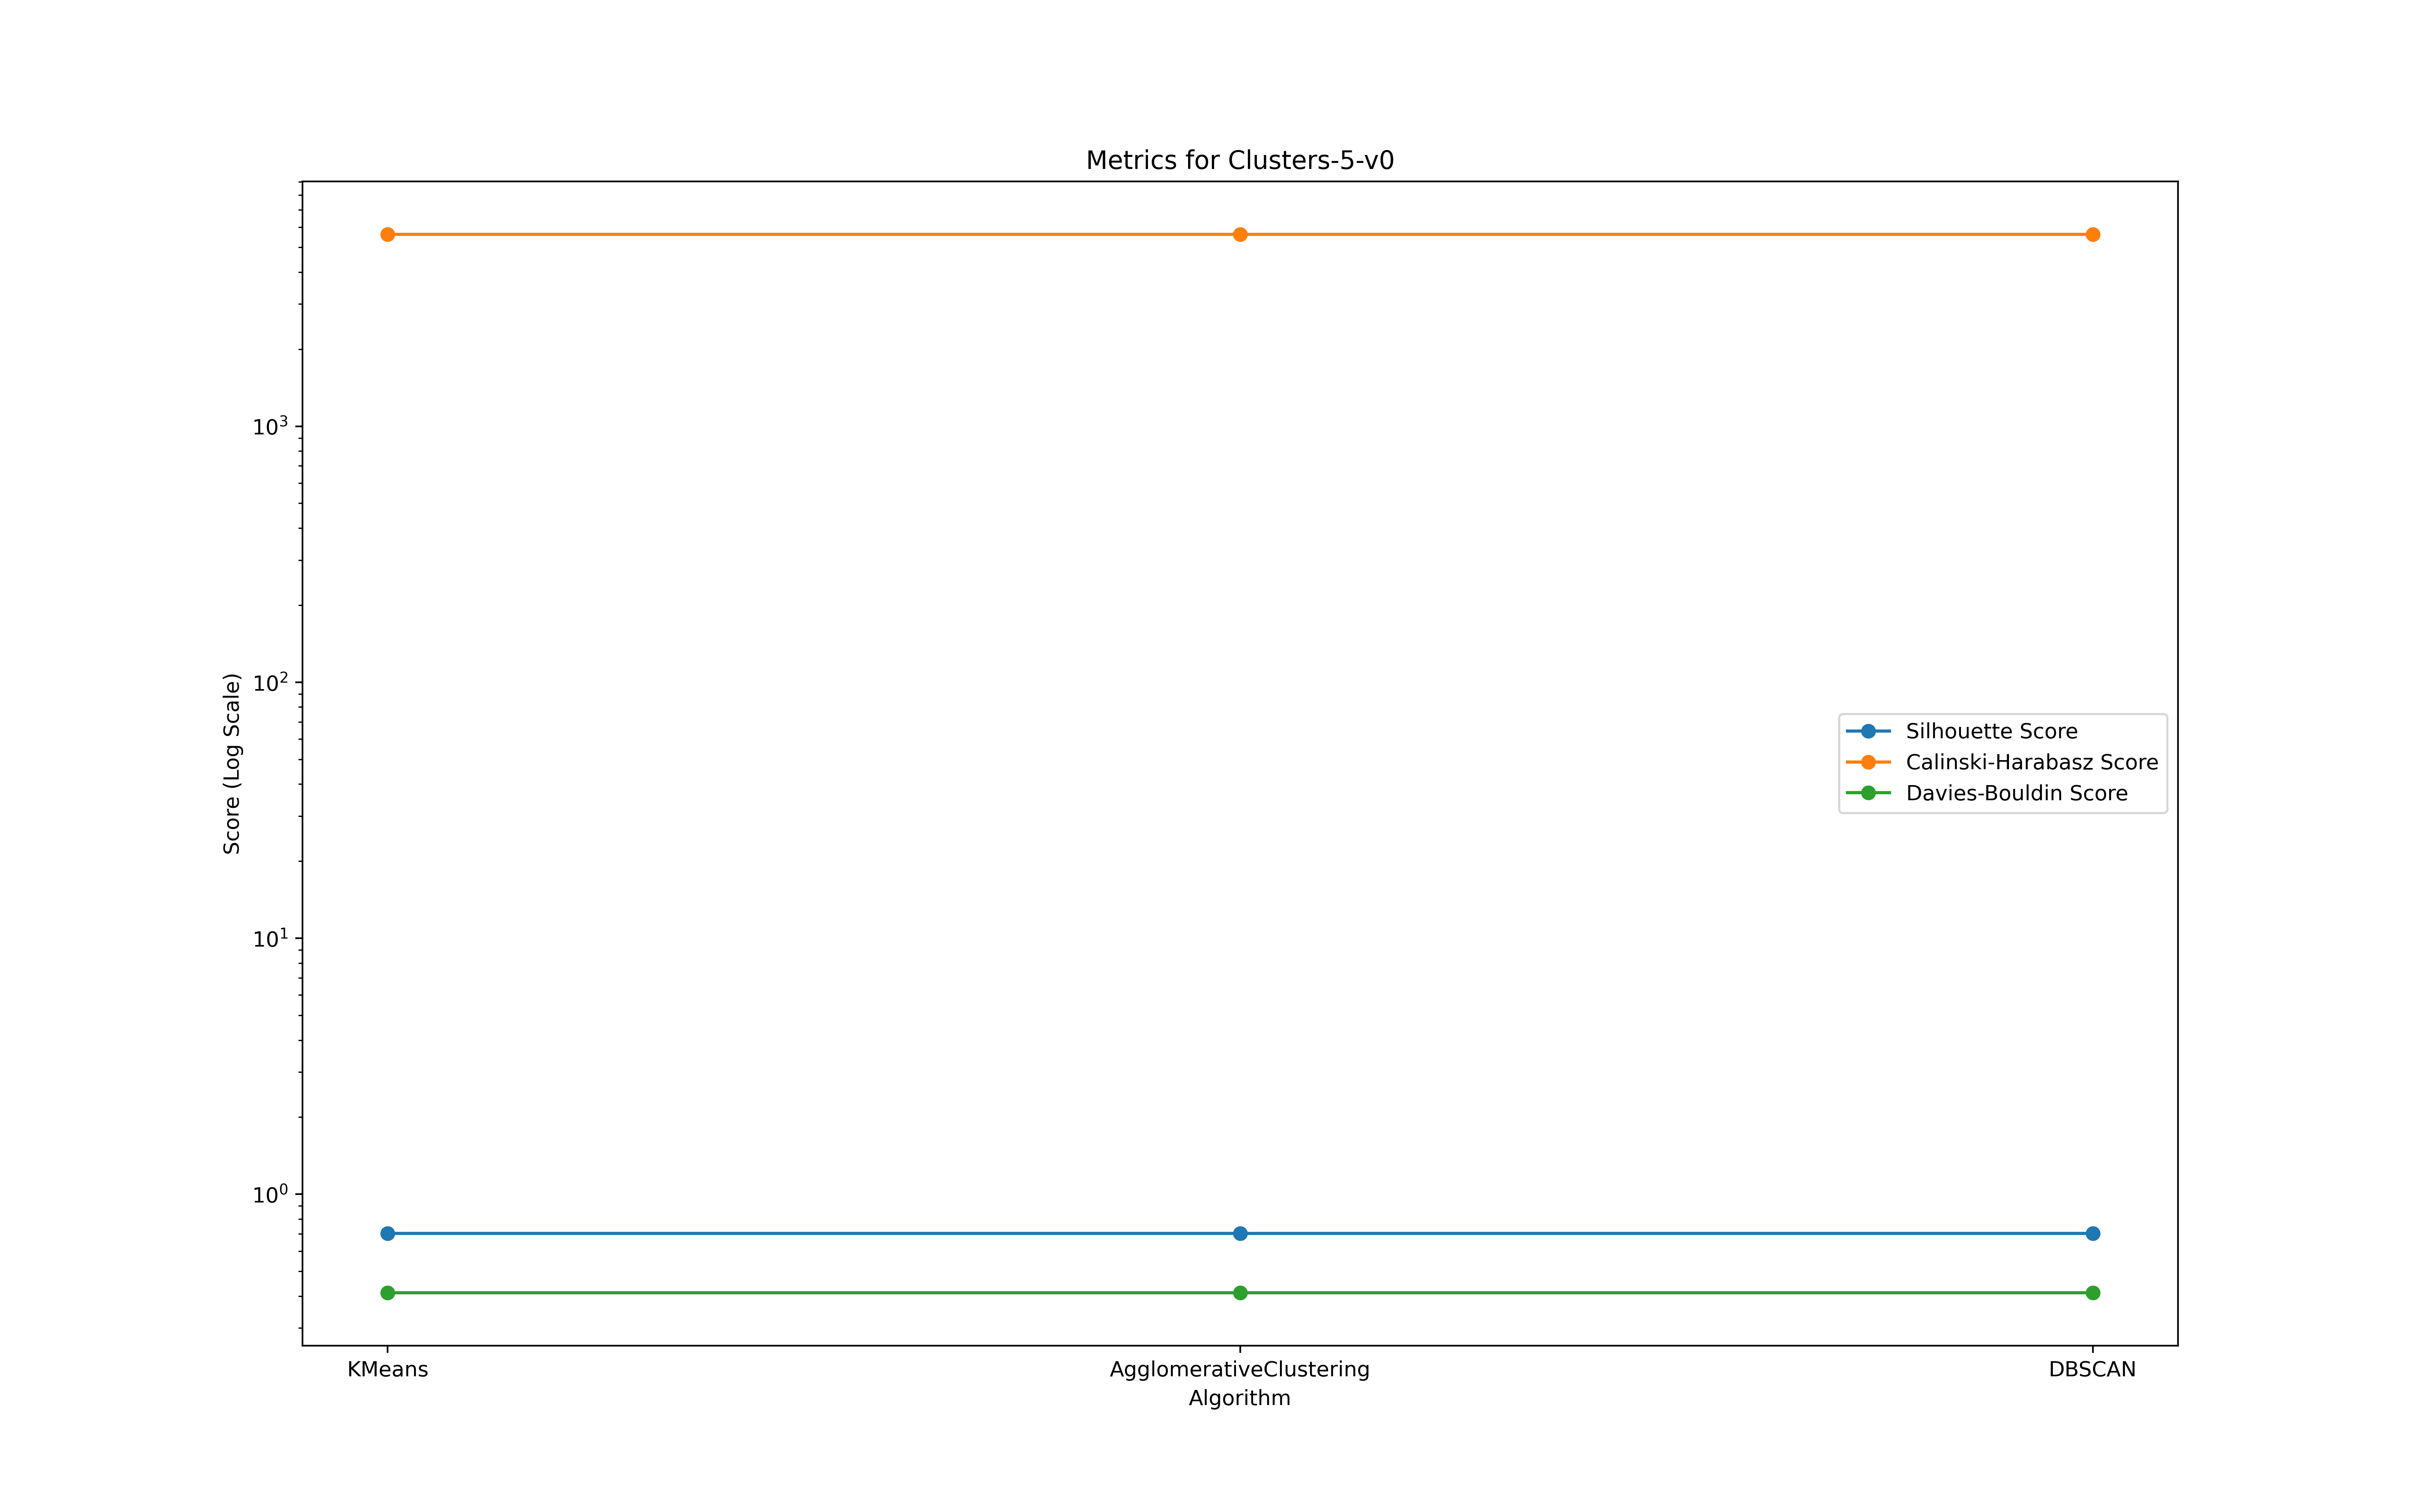
\includegraphics[width=0.8\linewidth]{Metrics/Clusters-5-v0-metrics.png}
	\caption{Dataset 1: Clustering Metrics}
	\label{fig:clusters-5-v0-metrics}
\end{figure}

\begin{figure}[H]
	\centering
	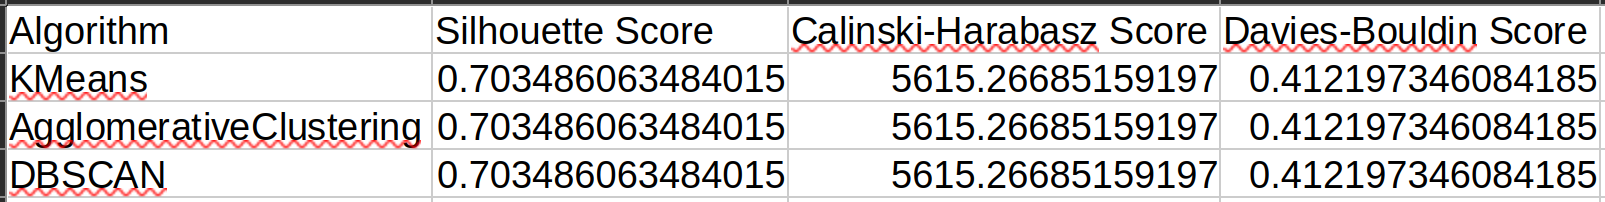
\includegraphics[width=0.9\linewidth]{Metrics/dataset-1.png}
	\caption{Dataset 1: Clustering Metrics}
	\label{fig:dataset-1}
\end{figure}

The error metrics for all 3 algorithms are exactly the same, indicating that the clustering quality is consistent across the algorithms. The Silhouette Scores are high, indicating well-separated clusters. The Calinski-Harabasz Scores are also high, suggesting compact and well-separated clusters. The Davies-Bouldin Scores are low, indicating good cluster similarity.

\subsection*{Dataset 2}

\begin{figure}[H]
	\centering
	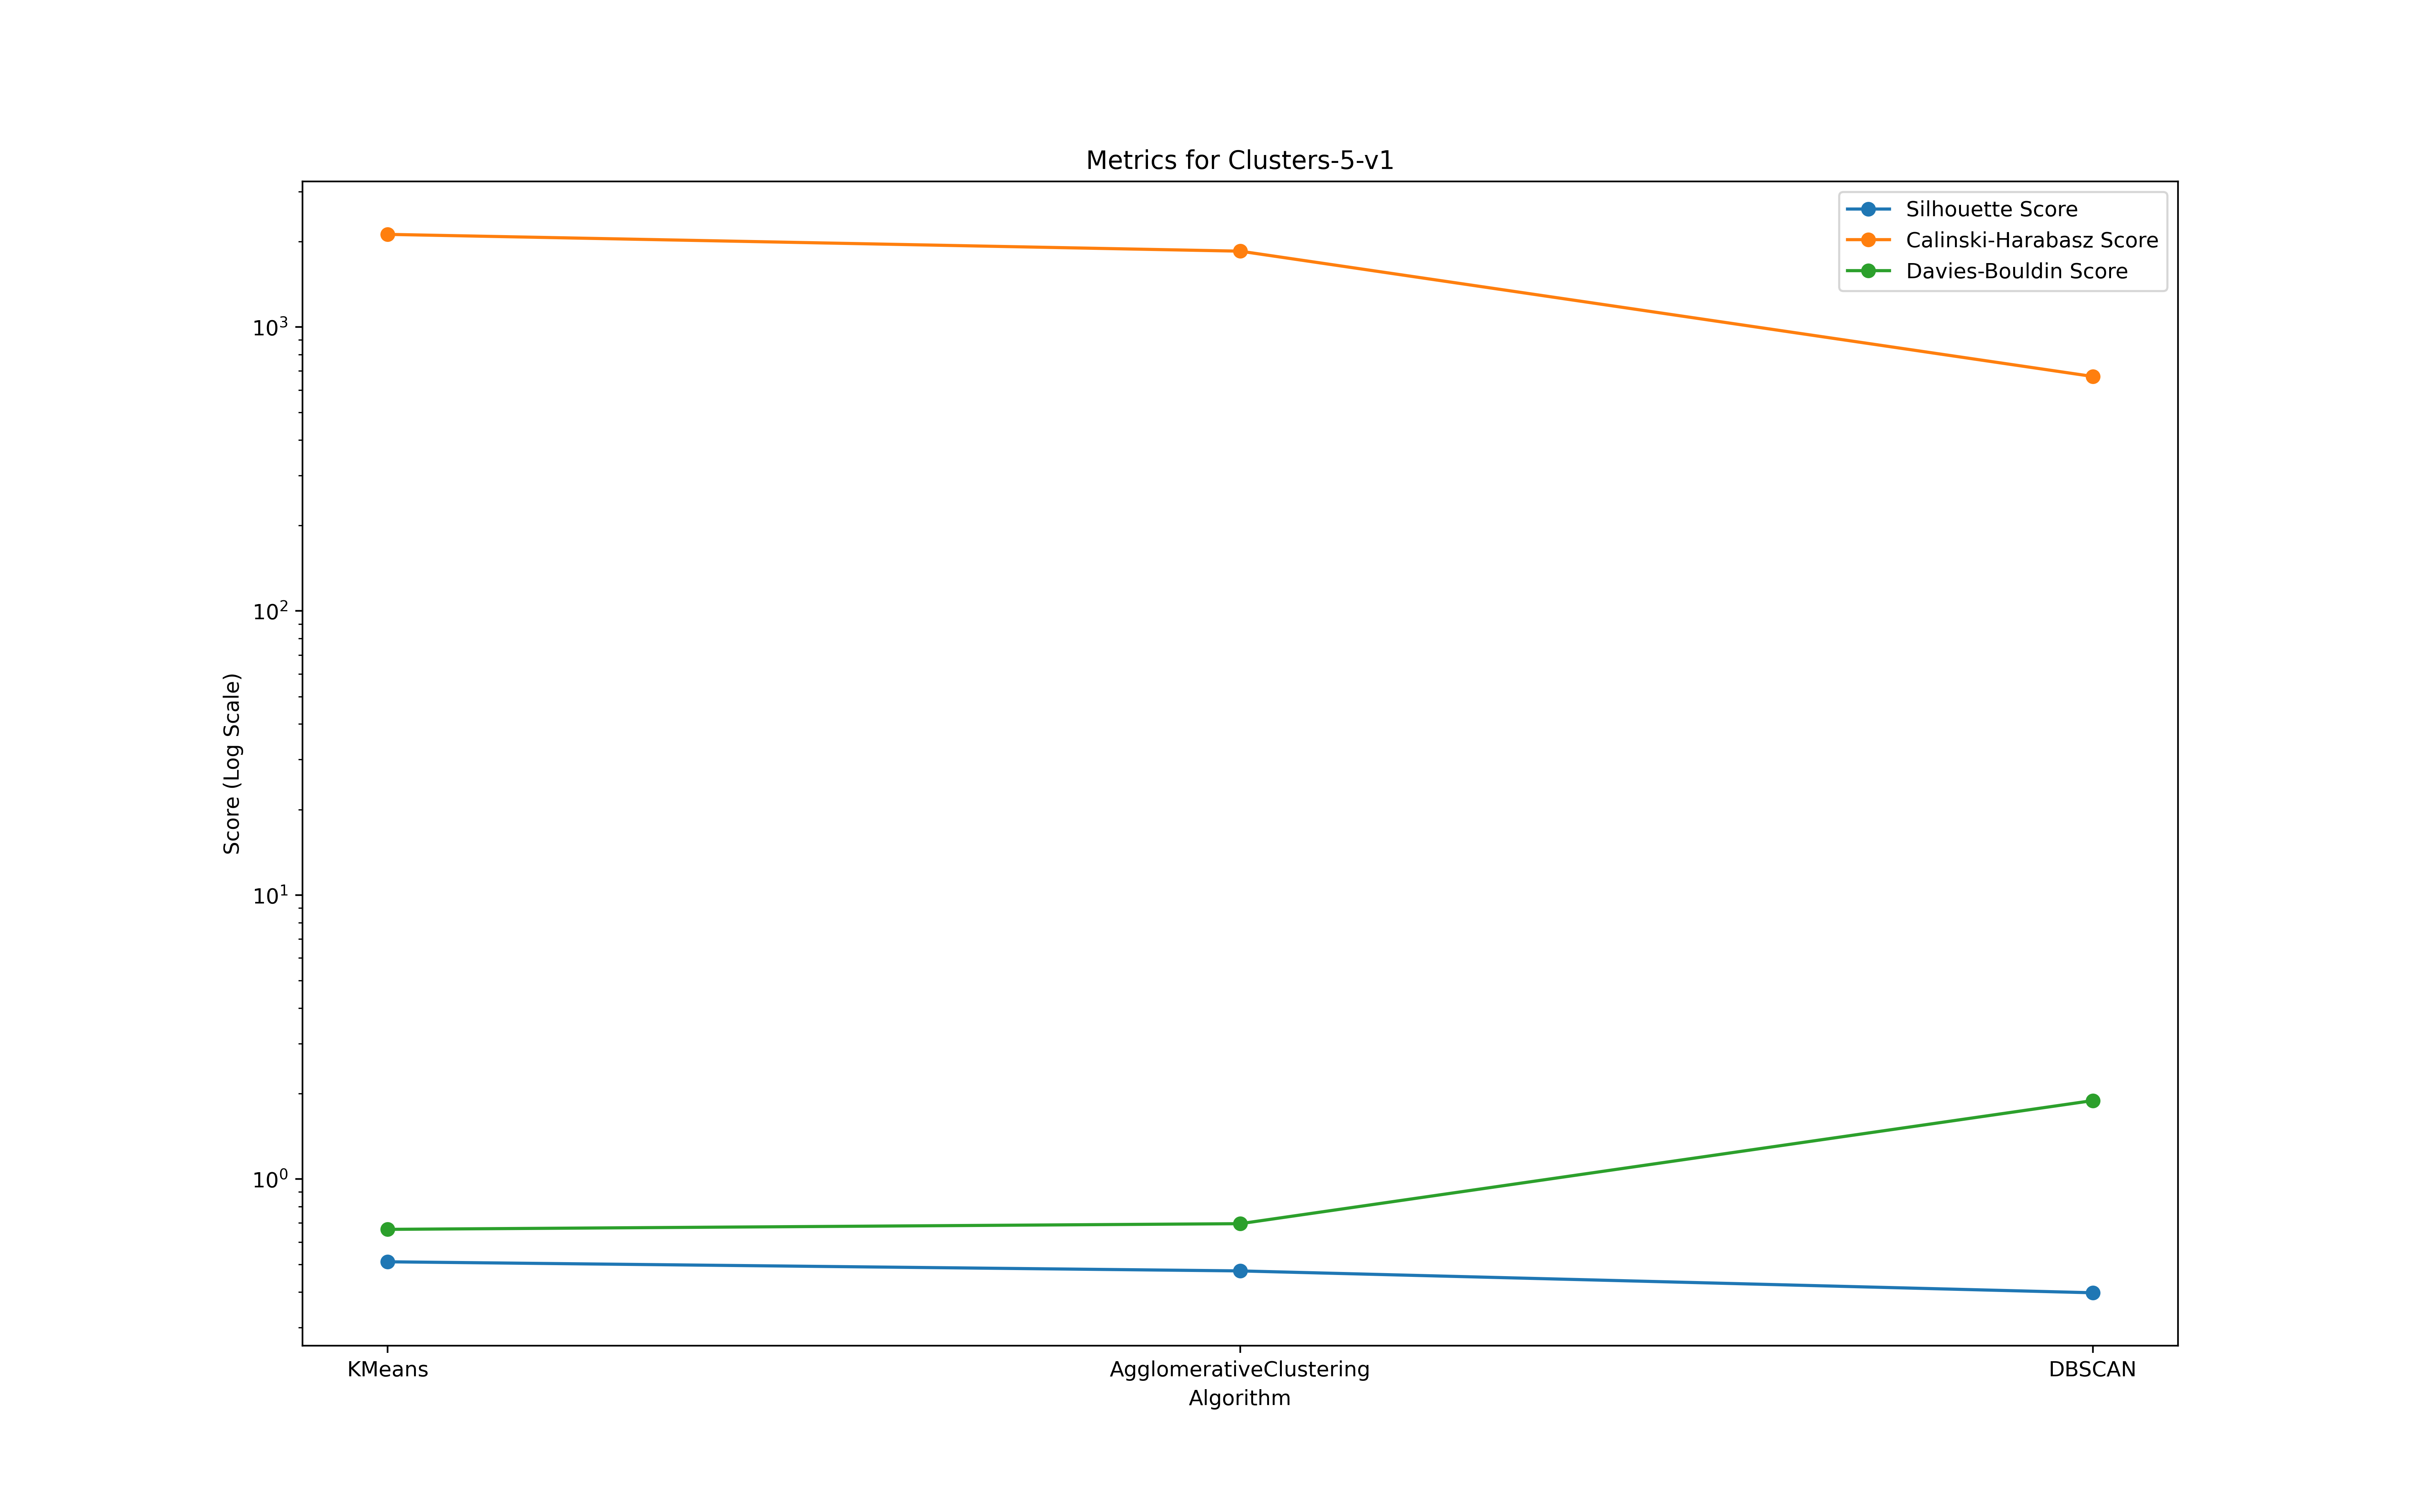
\includegraphics[width=0.8\linewidth]{Metrics/Clusters-5-v1-metrics.png}
	\caption{Dataset 2: Clustering Metrics}
	\label{fig:clusters-5-v1-metrics}
\end{figure}

\begin{figure}[H]
	\centering
	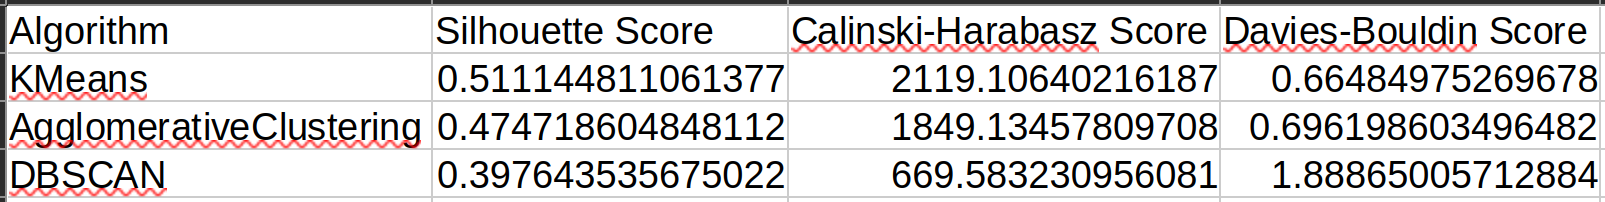
\includegraphics[width=0.9\linewidth]{Metrics/dataset-2.png}
	\caption{Dataset 2: Clustering Metrics}
	\label{fig:dataset-2}
\end{figure}

The Silhouette Scores for the 3 algorithms reduces as we go from K-Means to Agglomerative to DBSCAN. This indicates that the clusters are less well-separated in Dataset 2 compared to Dataset 1. The Calinski-Harabasz Scores also decrease, suggesting less compact clusters. The Davies-Bouldin Scores increase, indicating higher cluster similarity.

\subsection*{Dataset 3}

\begin{figure}[H]
	\centering
	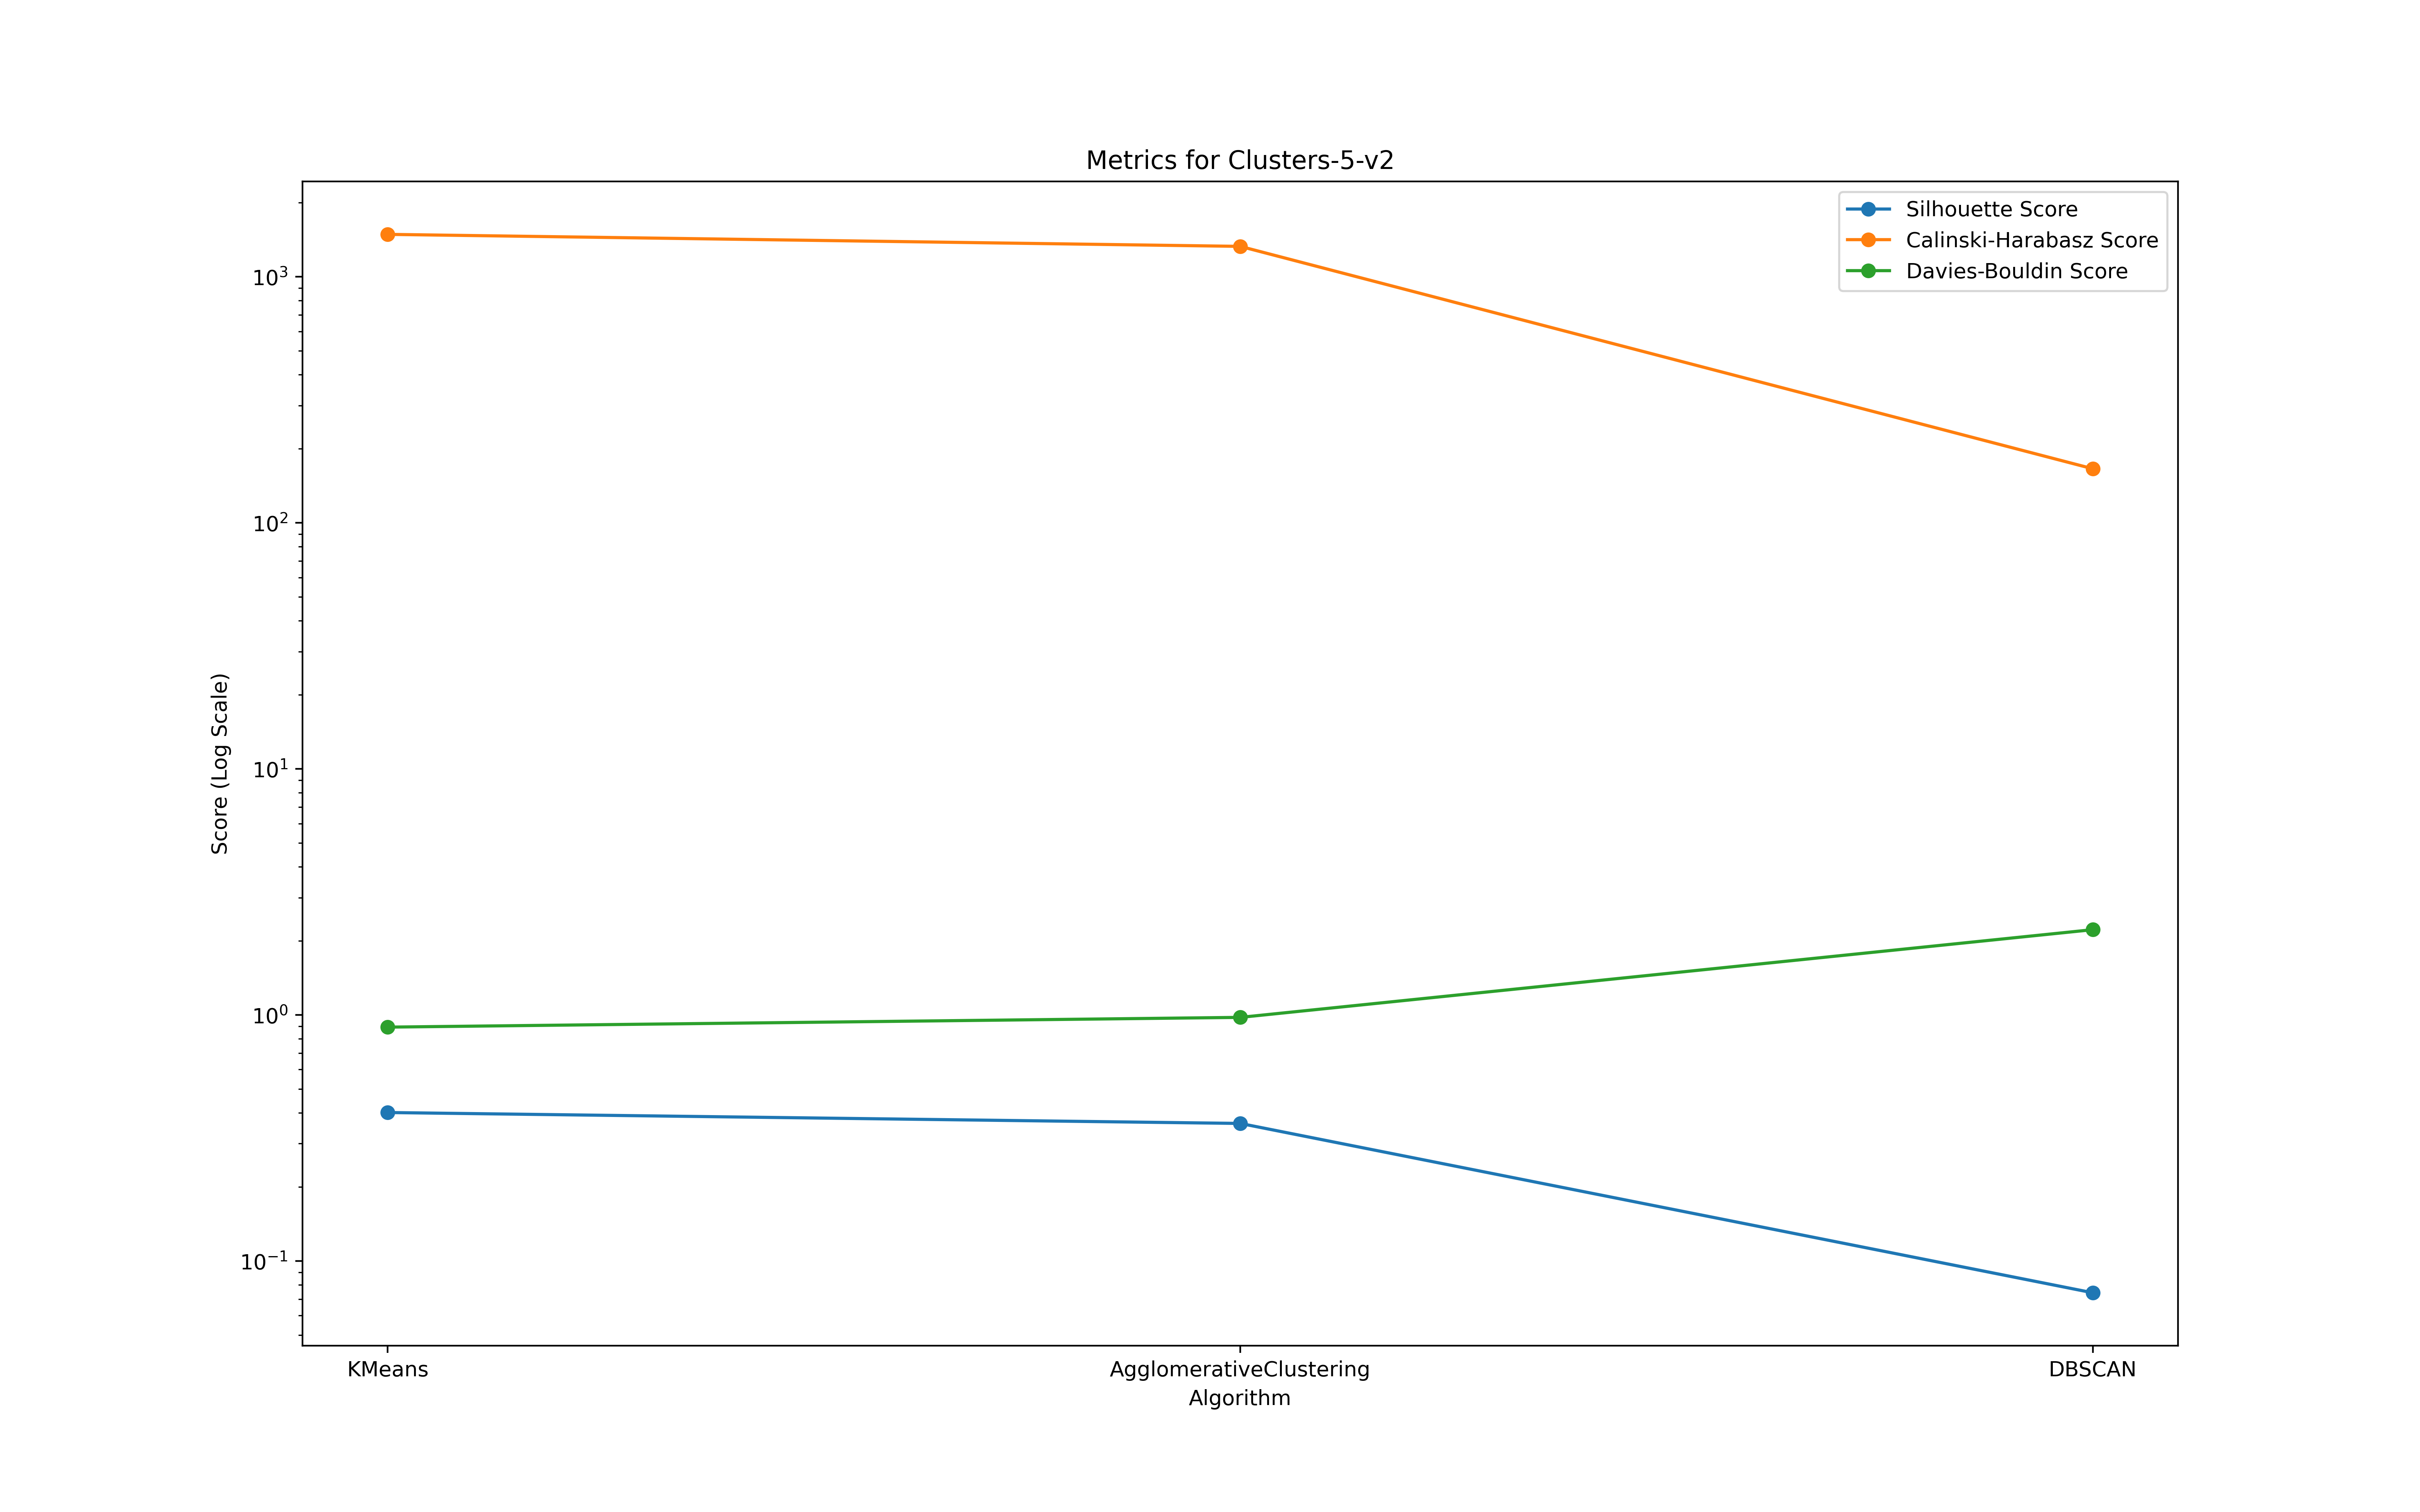
\includegraphics[width=0.8\linewidth]{Metrics/Clusters-5-v2-metrics.png}
	\caption{Dataset 3: Clustering Metrics}
	\label{fig:clusters-5-v2-metrics}
\end{figure}

\begin{figure}[H]
	\centering
	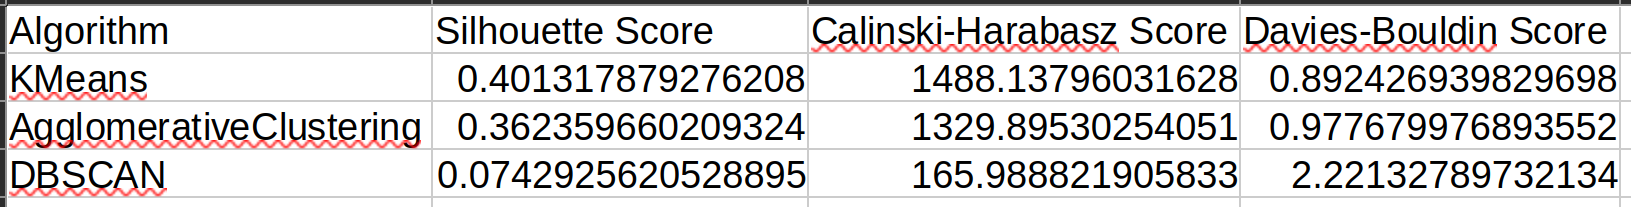
\includegraphics[width=0.9\linewidth]{Metrics/dataset-3.png}
	\caption{Dataset 3: Clustering Metrics}
	\label{fig:dataset-3}
\end{figure}

The Silhouette Scores for Dataset 3 are significantly lower than the other datasets, indicating poor cluster separation. The Calinski-Harabasz Scores are also the lowest, reflecting less compact clusters. The Davies-Bouldin Scores are the highest, showing higher cluster similarity. \\

The Silhouette Scores for each dataset and clustering algorithm provide insights into the clustering quality. In Dataset Clusters-5-v0.csv, all algorithms show high Silhouette Scores, indicating well-separated clusters. For Clusters-5-v1.csv, scores are slightly lower, reflecting some overlap. In Clusters-5-v2.csv, scores are significantly lower, indicating poor separation. \\

The Calinski-Harabasz Scores demonstrate the compactness and separation of clusters. Dataset Clusters-5-v0.csv exhibits high scores across algorithms, suggesting well-defined clusters. Scores for Clusters-5-v1.csv are lower, and for Clusters-5-v2.csv, they are the lowest, showing that clusters are not well-separated. \\

The Davies-Bouldin Scores highlight the average similarity of clusters. For Dataset Clusters-5-v0.csv, all algorithms achieve low scores, indicating distinct clusters. For Clusters-5-v1.csv, the scores are higher, suggesting some cluster overlap. Clusters-5-v2.csv shows the highest Davies-Bouldin Scores, reflecting significant cluster mixing. \\


\clearpage